
%
\section{Results} % (fold)
\label{sec:fst_results}
%
We tested our algorithm on an analytic test function that is designed to
resemble the behavior of a vortex, and on two real-world simulations.
%
The simulations were carried out on Phase 1 of the SuperMUC Petascale System of
the Leibnitz Supercomputing Centre in Garching, Germany.
%
Each node of the system has two 8-core Intel Xeon E5 processors with a clock
frequency of \SI{2.7}{\giga\hertz} and \SI{32}{\giga\byte} of shared memory.
%
The nodes are connected via Infiniband FDR10.
%

%
In the following sections, we evaluate the accuracy of our method on the
analytic test function, and show our results for the two simulation cases.
%

%
\subsection{Analytical Test Function} % (fold)
\label{sub:analytic_test_function}
%
\begin{figure*}
    \centering
    \setlength{\figurewidth}{\textwidth}
    %
%

\begin{tikzpicture}[
    font=\small,
    thick,
    mydash/.style={dashed, dash phase=-1.5pt},
    label/.style={align=left, inner sep=0},
    image/.style={inner sep=0, outer sep=0, node distance = 0 and 0}
]
    \pgfplotsset{colormap={warm}{
    rgb=(1, 1, 1)
    rgb=(0.98823499999999997, 0.98039200000000004, 0.87058800000000003)
    rgb=(0.99215699999999996, 0.96470599999999995, 0.71372500000000005)
    rgb=(0.98823499999999997, 0.95686300000000002, 0.64313699999999996)
    rgb=(0.98039200000000004, 0.91764699999999999, 0.50980400000000003)
    rgb=(0.96862700000000002, 0.87451000000000001, 0.40784300000000001)
    rgb=(0.94901999999999997, 0.82352899999999996, 0.32156899999999999)
    rgb=(0.92941200000000002, 0.77647100000000002, 0.27843099999999998)
    rgb=(0.90980399999999995, 0.71764700000000003, 0.235294)
    rgb=(0.89019599999999999, 0.65882399999999997, 0.196078)
    rgb=(0.87843099999999996, 0.61960800000000005, 0.168627)
    rgb=(0.87058800000000003, 0.54901999999999995, 0.156863)
    rgb=(0.85097999999999996, 0.47450999999999999, 0.145098)
    rgb=(0.83137300000000003, 0.41176499999999999, 0.13333300000000001)
    rgb=(0.81176499999999996, 0.34509800000000002, 0.11372500000000001)
    rgb=(0.78823500000000002, 0.26666699999999999, 0.094117599999999996)
    rgb=(0.74117599999999995, 0.18431400000000001, 0.074509800000000001)
    rgb=(0.69019600000000003, 0.12548999999999999, 0.062745099999999998)
    rgb=(0.61960800000000005, 0.062745099999999998, 0.043137300000000003)
    rgb=(0.54901999999999995, 0.027451, 0.070588200000000004)
    rgb=(0.47058800000000001, 0.0156863, 0.090196100000000001)
    rgb=(0.40000000000000002, 0.0039215700000000001, 0.101961)
    rgb=(0.34902, 0, 0.129412)
}}

    % \node[image] (image1)
    % {
    %     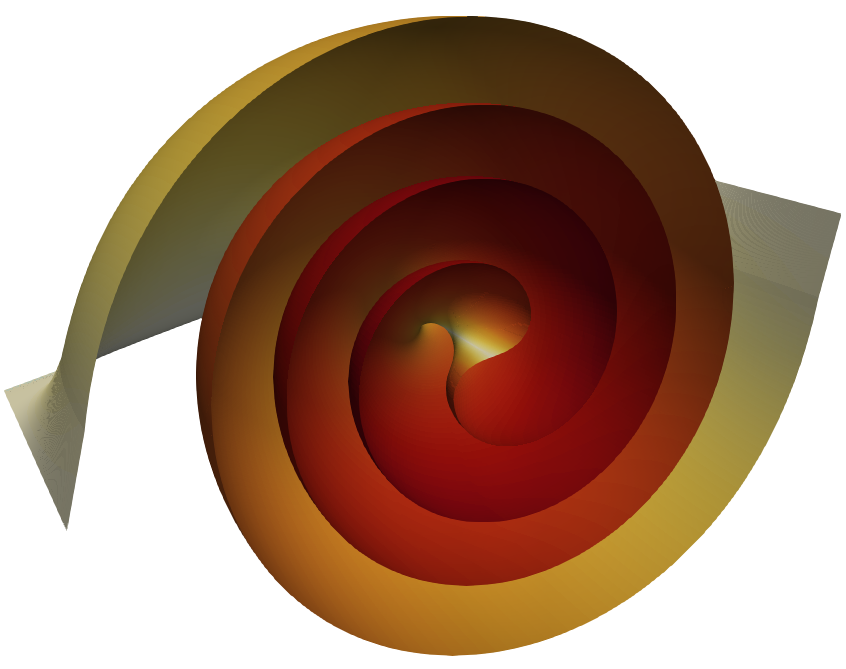
\includegraphics[width=0.5\figurewidth]{figures/ground_truth_log_highres}%
    % };
    % \node[anchor=north] at (image1.south) {\small ground truth};

    \node[image] (image2)
    {
        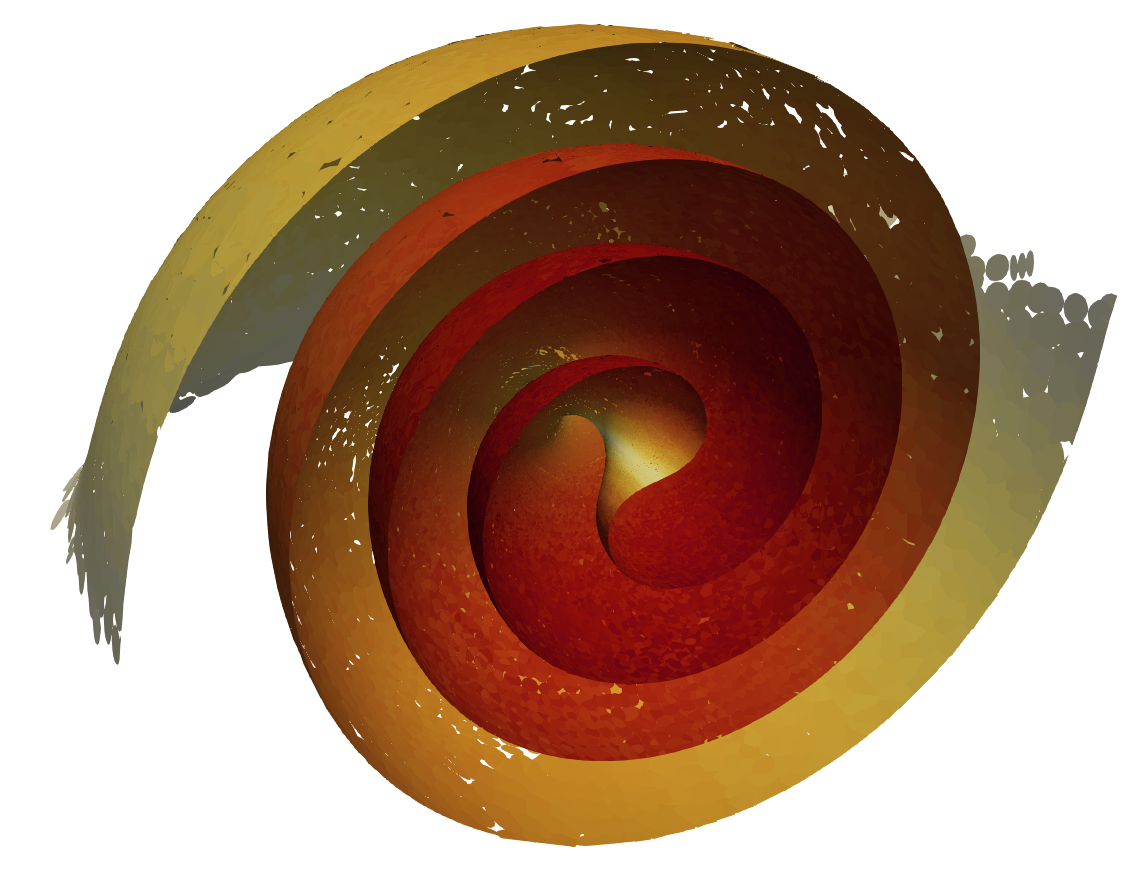
\includegraphics[width=0.5\figurewidth]{figures/norm_0_5_tan_0_01_log}%
    };
    \begin{scope}
        \clip (image2.south) -- (image2.south west) -- (image2.north west) --
            (image2.north);
        \node[image] (gt1) at (image2)
        {
            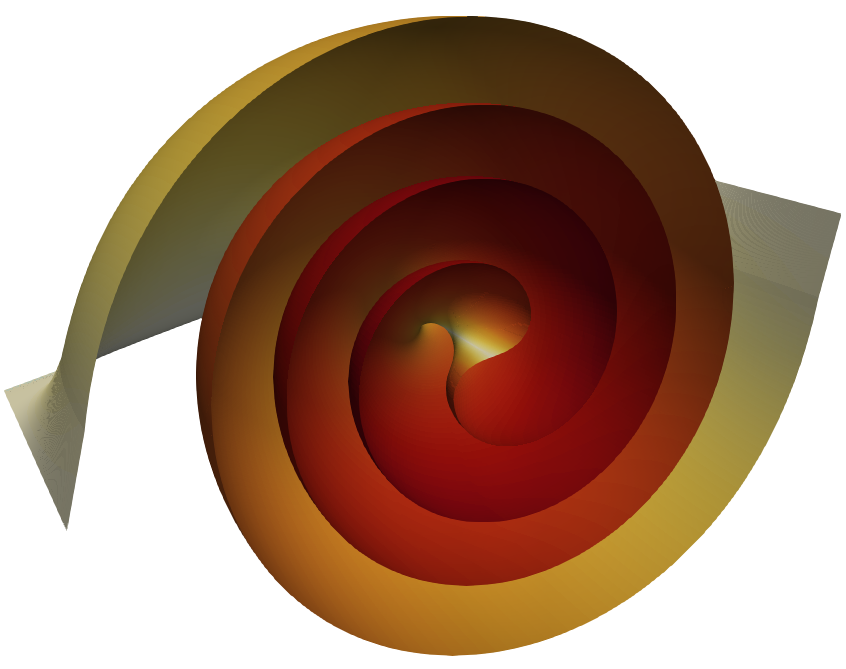
\includegraphics[width=0.5\figurewidth]{figures/ground_truth_log_highres}%
        };
    \end{scope}
    \draw[mydash] (image2.south) -- (image2.north);
    \node[label, anchor=east] at (image2.south east)
    {
        $
        \begin{aligned}
                r_\shortparallel &= 0.01 \\
                N &= \num{143.5}\si{\kilo}
        \end{aligned}
        $
    };
    % \node[label, anchor=south west] at (image2.south west) {ground\\truth};


    \node[image, right=of image2] (image3)
    {
        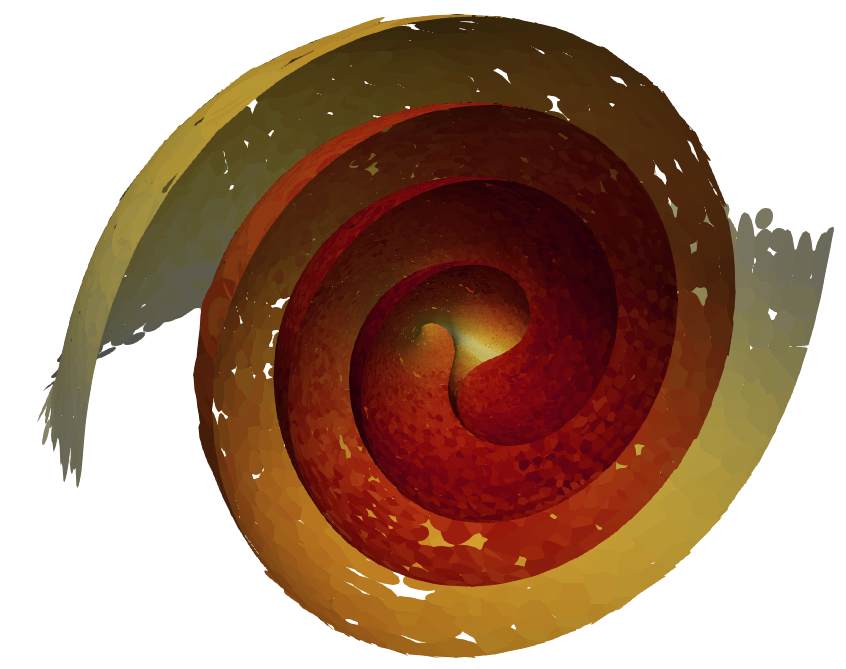
\includegraphics[width=0.5\figurewidth]{figures/norm_0_5_tan_0_02_log}%
    };
    \begin{scope}
        \clip (image3.south) -- (image3.south west) -- (image3.north west) --
            (image3.north);
        \node[image] (gt1) at (image3)
        {
            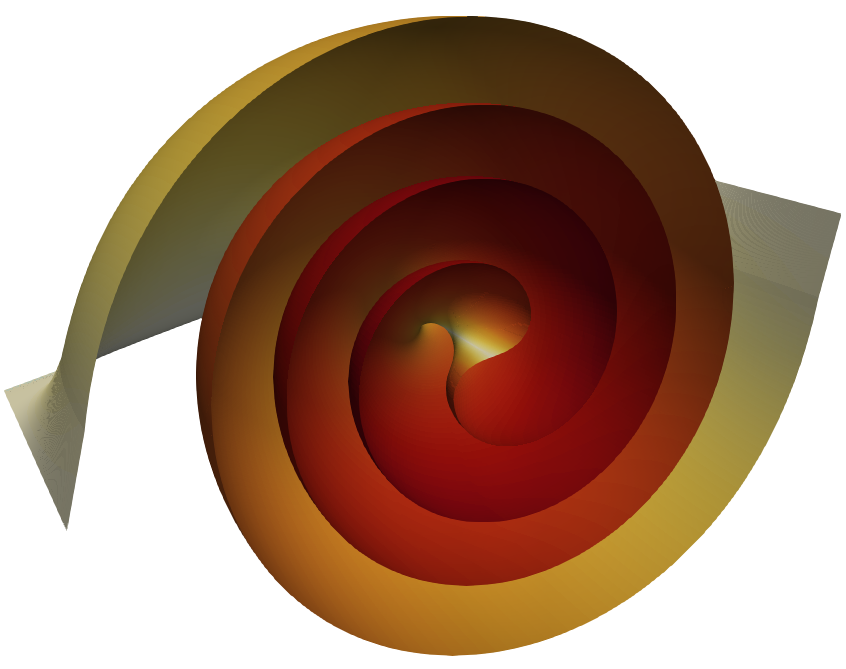
\includegraphics[width=0.5\figurewidth]{figures/ground_truth_log_highres}%
        };
    \end{scope}
    \draw[mydash] (image3.south) -- (image3.north);
    \node[anchor=east] at (image3.south east)
    {
        $
        \begin{aligned}
                r_\shortparallel &= 0.02 \\
                N &= \num{58.1}\si{\kilo}
        \end{aligned}
        $
    };
    % \node[label, anchor=south west] at (image3.south west) {ground\\truth};


    \node[image, below=0.5cm of image2] (image4)
    {
        
\includegraphics[width=0.5\figurewidth]{figures/norm_0_5_tan_0_05_log}%
    };
    \begin{scope}
        \clip (image4.south) -- (image4.south west) -- (image4.north west) --
            (image4.north);
        \node[image] (gt1) at (image4)
        {
            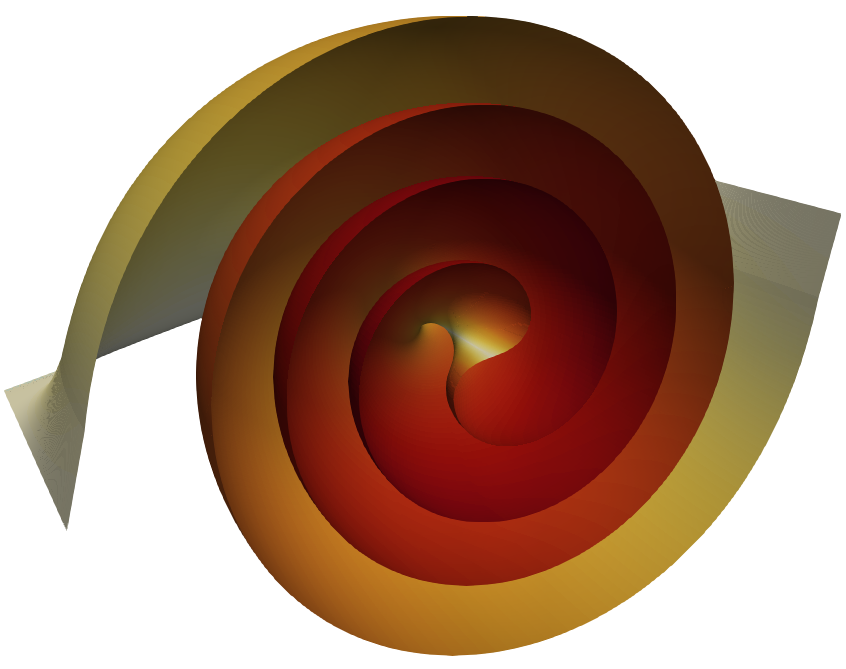
\includegraphics[width=0.5\figurewidth]{figures/ground_truth_log_highres}%
        };
    \end{scope}
    \draw[mydash] (image4.south) -- (image4.north);
    \node[anchor=east] at (image4.south east)
    {
        $
        \begin{aligned}
                r_\shortparallel &= 0.05 \\
                N &= \num{15.4}\si{\kilo}
        \end{aligned}
        $
    };
    % \node[label, anchor=south west] at (image4.south west) {ground\\truth};


    \node[image, right=of image4] (image5)
    {
        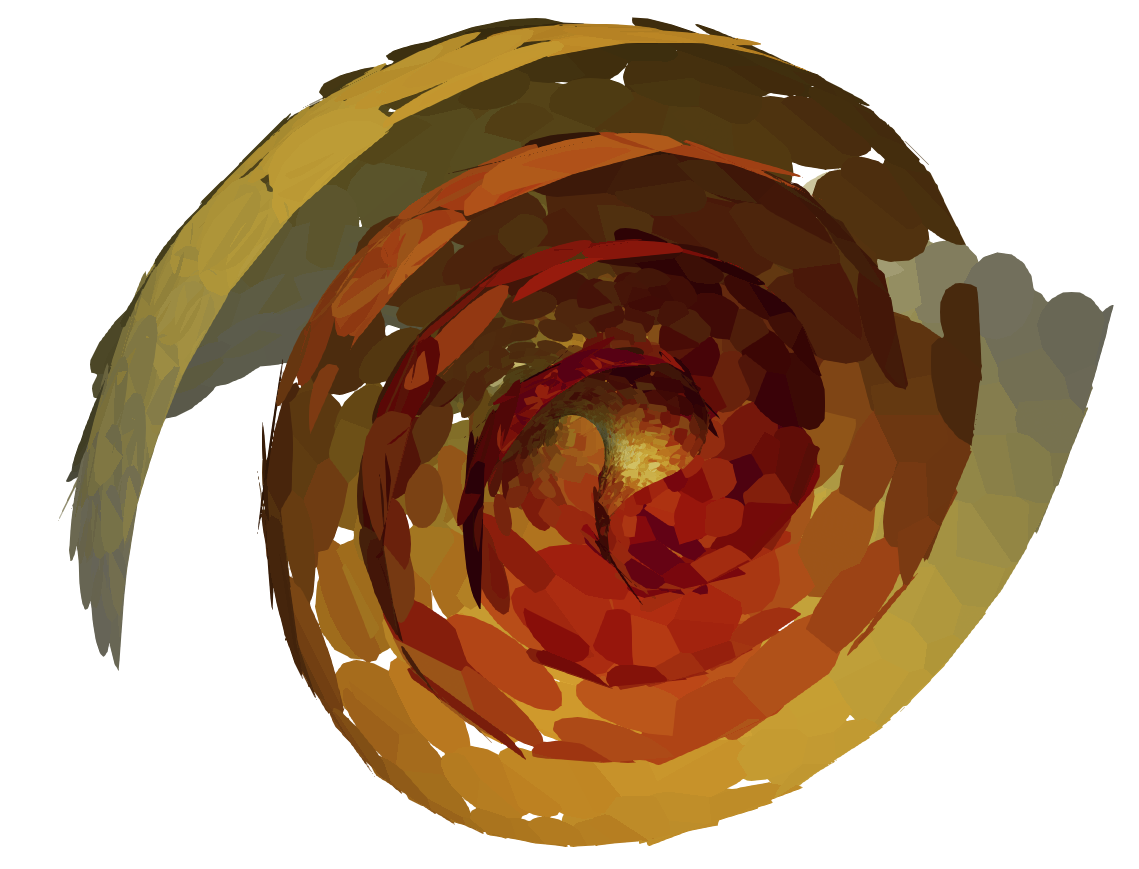
\includegraphics[width=0.5\figurewidth]{figures/norm_0_5_tan_0_1_log}%
    };
    \begin{scope}
        \clip (image5.south) -- (image5.south west) -- (image5.north west) --
            (image5.north);
        \node[image] (gt1) at (image5)
        {
            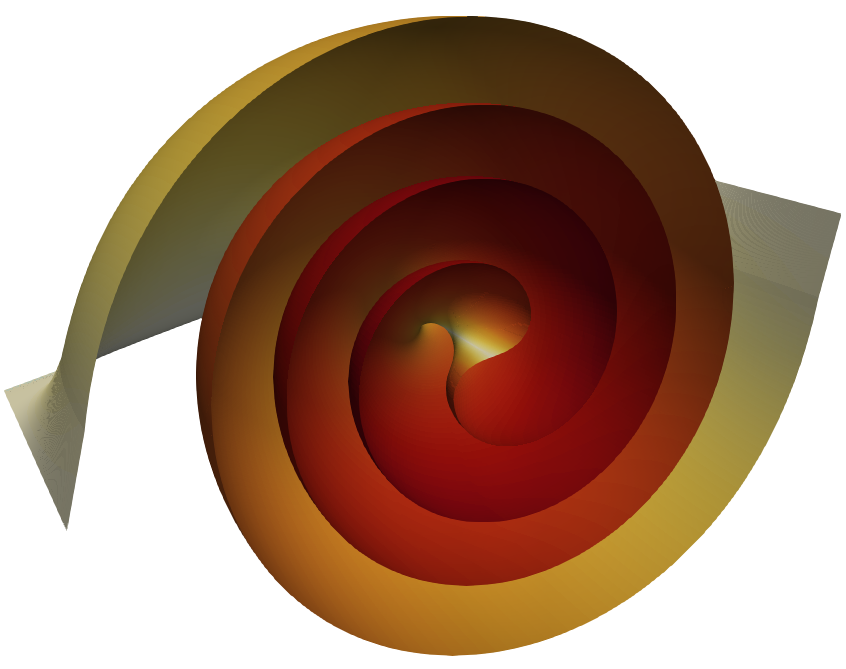
\includegraphics[width=0.5\figurewidth]{figures/ground_truth_log_highres}%
        };
    \end{scope}
    \draw[mydash] (image5.south) -- (image5.north);
    \node[anchor=east] at (image5.south east)
    {
        $
        \begin{aligned}
                r_\shortparallel &= 0.1 \\
                N &= \num{5}\si{\kilo}
        \end{aligned}
        $
    };
    % \node[label, anchor=south west] at (image5.south west) {ground\\truth};


    \node[anchor=north east, yshift=-0.5cm]
        at (image5.south east){
        \begin{axis}[
            scale only axis,
            height=3cm,
            hide axis,
            domain=0:2.1,
            % xmode=log,
            colorbar horizontal,
            colorbar/width=0.25cm,
            colormap name={warm},
            point meta min=0, point meta max=2.1,
            colorbar style={
                title=$c$,
                scaled ticks=false,
                % xmode=log,
                xtick={0, 1, 2},
                xticklabels = {$10^{\,0}$, $10^{\,1}$, $10^{\,2}$}
            }]
          \end{axis}
    };

\end{tikzpicture}
    \caption{The number of patches $N$ and the stretch coefficient $c$ of the
         tangential deformation gradient $\hat\mF_{\,0}^{\,2}$ for the analytic
         test function, using $r_\perp = 0.5$ and varying values for
         $r_\shortparallel$. Each micro-patch is represented by an ellipse
         scaled and aligned according to its principal axes and orthgonal to its
         surface normal.}
    \label{fig:ground_truth_comparison}
\end{figure*}
%
\begin{figure}
    \centering
    % \begin{captionbeside}
        % {Box plot of error distributions for the analytical test function.
         % We show the minimum, lower quartile, median, upper quartile and
         % maximum errors for different values of $r_\shortparallel$.}
        \setlength\figurewidth{0.9\linewidth}
        %
% Commented out values show differences of log10'ed maximum stretch values
%
\begin{tikzpicture}%[scale=\figurewidth/1cm*0.05]
\begin{axis}[
    small,
    width=1.0\figurewidth,
    height=0.6\figurewidth,
    boxplot/draw direction=y,
    boxplot/box extend=0.008,
    xtick={0.01, 0.02, 0.05, 0.1},
    scaled x ticks=false,
    x tick label style={/pgf/number format/fixed},
    xlabel near ticks,
    xlabel={$r_\shortparallel$},
    ylabel={Error},
    ylabel near ticks,
    extra y ticks=0,
    extra y tick style={grid=major},
    every tick/.style={color=black, thin},
]
% \addplot +[
%     mycolor1,
%     thick,
%     forget plot,
%     boxplot prepared={
%         % average=-0.1209,
%         draw position=0.01,
%         lower whisker=-0.4754,
%         lower quartile=-0.0448,
%         median=-0.0018,
%         upper quartile=0.0481,
%         upper whisker=0.5447
%     }
% ] coordinates{};

\addplot +[
    mycolor1,
    % thick,
    forget plot,
    boxplot prepared={
        % average=-0.1209,
        draw position=0.01,
        lower whisker=-13.9811,
        lower quartile=-0.3176,
        median=0.0185,
        upper quartile= 1.2833,
        upper whisker= 38.4859
    }
] coordinates{};

% \addplot +[
%     mycolor1,
%     thick,
%     forget plot,
%     boxplot prepared={
%         % average=-0.1209,
%         draw position=0.02,
%         lower whisker=-0.6230,
%         lower quartile=-0.0742,
%         median=-0.0096,
%         upper quartile=0.0663,
%         upper whisker=0.8500
%     }
% ] coordinates{};

\addplot +[
    mycolor1,
    % thick,
    forget plot,
    boxplot prepared={
        % average=-0.1209,
        draw position=0.02,
        lower whisker=-23.9069,
        lower quartile=-0.5360,
        median= 0.0097,
        upper quartile= 1.6632,
        upper whisker=51.1135
    }
] coordinates{};

% \addplot +[
%     mycolor1,
%     thick,
%     forget plot,
%     boxplot prepared={
%         % average=-0.1209,
%         draw position=0.05,
%         lower whisker=-0.7818,
%         lower quartile=-0.1556,
%         median=-0.0455,
%         upper quartile=0.0524,
%         upper whisker=1.2208
%     }
% ] coordinates{};

\addplot +[
    mycolor1,
    % thick,
    forget plot,
    boxplot prepared={
        % average=-0.1209,
        draw position=0.05,
        lower whisker=-27.4750,
        lower quartile=-1.0062,
        median=-0.1040,
        upper quartile= 1.0829,
        upper whisker= 94.2205
    }
] coordinates{};

% \addplot +[
%     mycolor1,
%     thick,
%     forget plot,
%     boxplot prepared={
%         % average=-0.1209,
%         draw position=0.1,
%         lower whisker=-1.2460,
%         lower quartile=-0.2575,
%         median=-0.0991,
%         upper quartile=0.0057,
%         upper whisker=2.0031
%     }
% ] coordinates{};

\addplot +[
    mycolor1,
    % thick,
    forget plot,
    boxplot prepared={
        % average=-0.1209,
        draw position=0.1,
        lower whisker=-41.4414,
        lower quartile=-1.8953,
        median=-0.4120,
        upper quartile=0.2488,
        upper whisker=77.4248
    }
] coordinates{};
\end{axis}
\end{tikzpicture}
    % \end{captionbeside}
    \caption{Box plot of error distributions for the analytical test function.
             We show the minimum, lower quartile, median, upper quartile and
             maximum errors for different values of $r_\shortparallel$.}
    \label{fig:ground_truth_errors}
\end{figure}
%
To evaluate the accuracy of the tangential deformation gradient obtained by our
method, we designed an analytic test function.
%
It imitates the behavior of a vortex in the shear layer between two gas streams.
%
The test function $s$ is defined as
%
\begin{align}
	s(x, y, z, t) &=
	\begin{cases}
		z \cos A - (x - \frac{1}{2}) \sin A,
			& \text{for } \sqrt{{(x - \frac{1}{2})}^2 + z^2} < \dfrac{1}{2} \\
		z, &\text{else}
	\end{cases}\, \text{,}\\
	A(x, y, z, t) &=
		2\pi t \sin{
			\left({
				\frac{\pi}{2}
				\left({1 + \sqrt{4x^2 - 4x + 4z^2 + 1}}\right)
			}\right)
		}^2
		\sin(\pi y)^2\, \text{.}
\end{align}
%
The isosurface $s = 0$ coincides with the $xy$ plane at $t=0$.
%
As $t$ increases, the surface is curled up around the center at $(x,~y,~z) =
(\sfrac{1}{2},~\sfrac{1}{2},~0)$.
%
The underlying velocity field of a vortex can not be easily expressed as an
analytic function.
%
We therefore assume a fluid velocity of $\vv = \vNull$ for our tests.
%

%
We observe the function in the domain ${x\in[0,~1]}$, ${y\in[0, 1]}$,
${z\in[-\sfrac{1}{2},~\sfrac{1}{2}]}$, ${t\in[0,~2]}$ resolved in a $72 \times
72 \times 72$ regular grid and a time step of $\Delta t = \num{5e-3}$.
%
This means that in the investigated time span the vortex makes exactly two full
turns, resolved in \num{4000} time steps.
%
This closely resembles the lifetime of a vortex and temporal resolution observed
in a real simulation setting.
%

%
The velocity $\vu$ of the surface $s = 0$ can be expressed as an analytic
function.
%
This enables us to obtain highly accurate ground truth data for the tangential
deformation gradient $\hat\mF$.
%
The largest singular value of $\hat\mF$ signifies the largest stretching
experienced by the local neighborhood of a point on the surface,
which we call the stretching coefficient $c$ with
%
\[
    c = \sigma_{\max}(\hat\mF)
      = \sqrt{\lambda_{\max}(\T{\hat\mF} \, \hat\mF)}\,\text{.}
\]
%
This is similar to the measure used when computing the \ac{FTLE} for measuring
separation in flow fields\cite{Haller2002}.
%
In all tests, we use a normal error threshold of $r_\perp = 0.5$, which is
rather coarse.
%
By doing this, we limit its influence on the accuracy of the results for
the tangential deformation.
%
We show the distribution of differences to the ground truth solution for
different tangential error thresholds $r_\shortparallel$ in
\autoref{fig:ground_truth_errors}.
%
For the sake of brevity, we only show the results for the complete interval
$t=[0,\,2]$, which will naturally show the largest errors.
%
\begin{figure}
    \centering
    \setlength{\figurewidth}{\textwidth}
    %
%
\begin{tikzpicture}[font=\small]
    \tikzstyle{image} = [anchor=center,
                         inner sep=0, outer sep=0,
                         node distance = 0.3cm and 0,
                         % draw=black,
                         minimum width=0.5\figurewidth]
    \tikzstyle{label} = [anchor=north,
                         align=left]
    \pgfplotsset{colormap={cooltowarm_extended}{
    rgb=(0.12548999999999999, 0, 0.38039200000000001)
    rgb=(0.11372500000000001, 0.023529399999999999, 0.45097999999999999)
    rgb=(0.105882, 0.050980400000000002, 0.50980400000000003)
    rgb=(0.039215699999999999, 0.039215699999999999, 0.56078399999999995)
    rgb=(0.031372499999999998, 0.098039200000000007, 0.59999999999999998)
    rgb=(0.043137300000000003, 0.16470599999999999, 0.63921600000000001)
    rgb=(0.054901999999999999, 0.24313699999999999, 0.67843100000000001)
    rgb=(0.054901999999999999, 0.31764700000000001, 0.70980399999999999)
    rgb=(0.050980400000000002, 0.39607799999999999, 0.74117599999999995)
    rgb=(0.039215699999999999, 0.466667, 0.76862699999999995)
    rgb=(0.031372499999999998, 0.53725500000000004, 0.78823500000000002)
    rgb=(0.031372499999999998, 0.61568599999999996, 0.81176499999999996)
    rgb=(0.023529399999999999, 0.70980399999999999, 0.83137300000000003)
    rgb=(0.050980400000000002, 0.80000000000000004, 0.85097999999999996)
    rgb=(0.070588200000000004, 0.85490200000000005, 0.87058800000000003)
    rgb=(0.26274500000000001, 0.90196100000000001, 0.86274499999999998)
    rgb=(0.42352899999999999, 0.94117600000000001, 0.87451000000000001)
    rgb=(0.57254899999999997, 0.96470599999999995, 0.83529399999999998)
    rgb=(0.65882399999999997, 0.98039200000000004, 0.84313700000000003)
    rgb=(0.764706, 0.98039200000000004, 0.86666699999999997)
    rgb=(0.82745100000000005, 0.98039200000000004, 0.88627500000000003)
    rgb=(0.91372500000000001, 0.98823499999999997, 0.93725499999999995)
    rgb=(1, 1, 1)
    rgb=(0.98823499999999997, 0.98039200000000004, 0.87058800000000003)
    rgb=(0.99215699999999996, 0.96470599999999995, 0.71372500000000005)
    rgb=(0.98823499999999997, 0.95686300000000002, 0.64313699999999996)
    rgb=(0.98039200000000004, 0.91764699999999999, 0.50980400000000003)
    rgb=(0.96862700000000002, 0.87451000000000001, 0.40784300000000001)
    rgb=(0.94901999999999997, 0.82352899999999996, 0.32156899999999999)
    rgb=(0.92941200000000002, 0.77647100000000002, 0.27843099999999998)
    rgb=(0.90980399999999995, 0.71764700000000003, 0.235294)
    rgb=(0.89019599999999999, 0.65882399999999997, 0.196078)
    rgb=(0.87843099999999996, 0.61960800000000005, 0.168627)
    rgb=(0.87058800000000003, 0.54901999999999995, 0.156863)
    rgb=(0.85097999999999996, 0.47450999999999999, 0.145098)
    rgb=(0.83137300000000003, 0.41176499999999999, 0.13333300000000001)
    rgb=(0.81176499999999996, 0.34509800000000002, 0.11372500000000001)
    rgb=(0.78823500000000002, 0.26666699999999999, 0.094117599999999996)
    rgb=(0.74117599999999995, 0.18431400000000001, 0.074509800000000001)
    rgb=(0.69019600000000003, 0.12548999999999999, 0.062745099999999998)
    rgb=(0.61960800000000005, 0.062745099999999998, 0.043137300000000003)
    rgb=(0.54901999999999995, 0.027451, 0.070588200000000004)
    rgb=(0.47058800000000001, 0.0156863, 0.090196100000000001)
    rgb=(0.40000000000000002, 0.0039215700000000001, 0.101961)
    rgb=(0.34902, 0, 0.129412)
}}
    \pgfplotsset{colormap={green_purple}{
    rgb=(0.23137254901960799, 0, 0.34509803921568599)
    rgb=(0.337254901960784, 0, 0.44313725490196099)
    rgb=(0.44705882352941201, 0, 0.54117647058823504)
    rgb=(0.60392156862745106, 0.015686274509803901, 0.65098039215686299)
    rgb=(0.76470588235294101, 0.035294117647058802, 0.76470588235294101)
    rgb=(0.88235294117647101, 0.21568627450980399, 0.82352941176470595)
    rgb=(1, 0.50980392156862697, 0.90588235294117603)
    rgb=(1, 0.76470588235294101, 0.95294117647058796)
    rgb=(1, 1, 1)
    rgb=(0.85882352941176499, 0.94901960784313699, 0.49803921568627502)
    rgb=(0.71764705882352897, 0.90196078431372595, 0)
    rgb=(0.54117647058823504, 0.82745098039215703, 0)
    rgb=(0.36470588235294099, 0.752941176470588, 0)
    rgb=(0.25490196078431399, 0.64313725490196105, 0)
    rgb=(0.149019607843137, 0.53725490196078396, 0)
    rgb=(0.074509803921568599, 0.40000000000000002, 0.023529411764705899)
    rgb=(0, 0.26300000000000001, 0.050999999999999997)
}}

    \node[image] (image1)
    {
        \begin{tikzpicture}
            \node[image] (base) at (0,0) {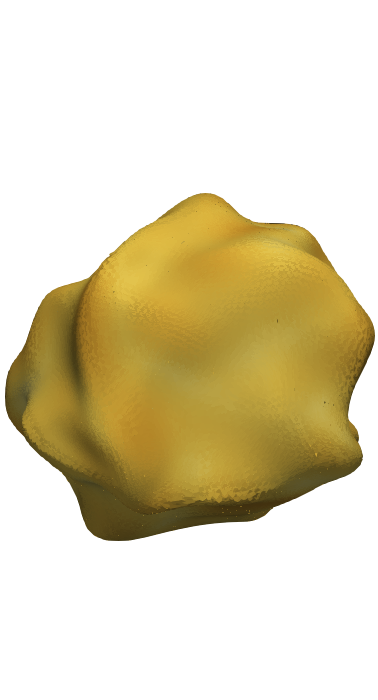
\includegraphics[height=0.45\figurewidth]{figures/spherical_time_1_02e-4}};%
            \begin{scope}
                \clip (base.south west) -- (base.north west) -- (base.north east) -- (base.south east) -- cycle;
                \clip (-2.0, -3.5) -- (2.0, 3.5) -- (4.0, 3.5) -- (4.0, -3.5)  -- cycle;
                \node[image] at (0,0) {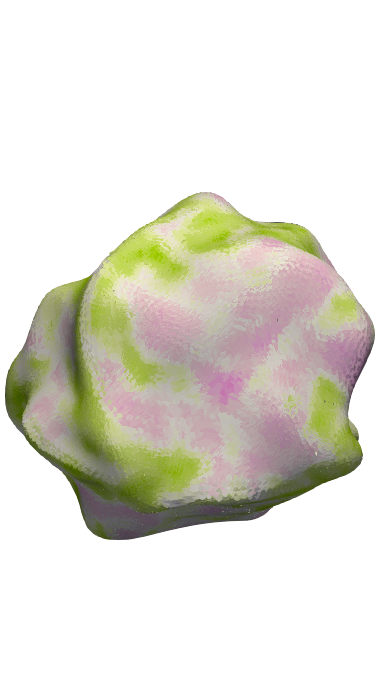
\includegraphics[height=0.45\figurewidth]{figures/spherical_time_1_02e-4_density_factor}};%
            \end{scope}
            \draw[thick, dashed, shorten <=2.1cm, shorten >=2.45cm] (-2.0, -3.5) -- (2.0, 3.5);
        \end{tikzpicture}
    };
    \node[label, yshift=1.3cm] at (image1.south) {$\begin{aligned}t &= \SI{1e-4}{\second} \\ N&=\num{50}\si{\kilo}\end{aligned}$};

    \node[image, right=of image1] (image2)
    {
        \begin{tikzpicture}
            \node[image] (base) {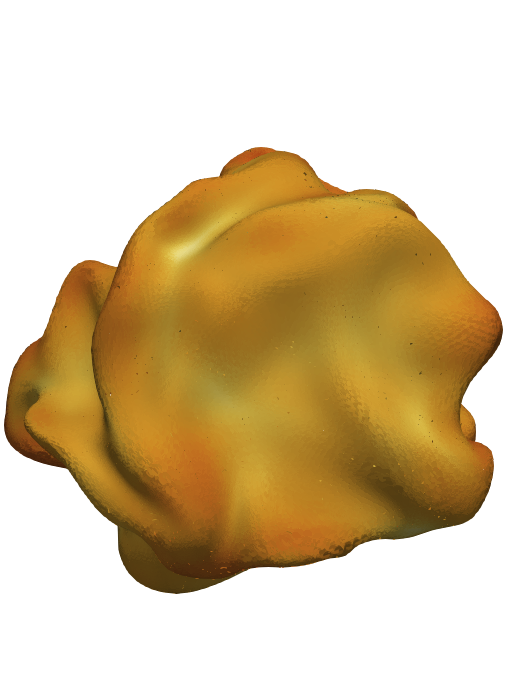
\includegraphics[height=0.45\figurewidth]{figures/spherical_time_1_7e-4}};%
            \begin{scope}
                \clip (base.south west) -- (base.north west) -- (base.north east) -- (base.south east) -- cycle;
                \clip (-2.0, -3.5) -- (2.0, 3.5) -- (4.0, 3.5) -- (4.0, -3.5)  -- cycle;
                \node[image] {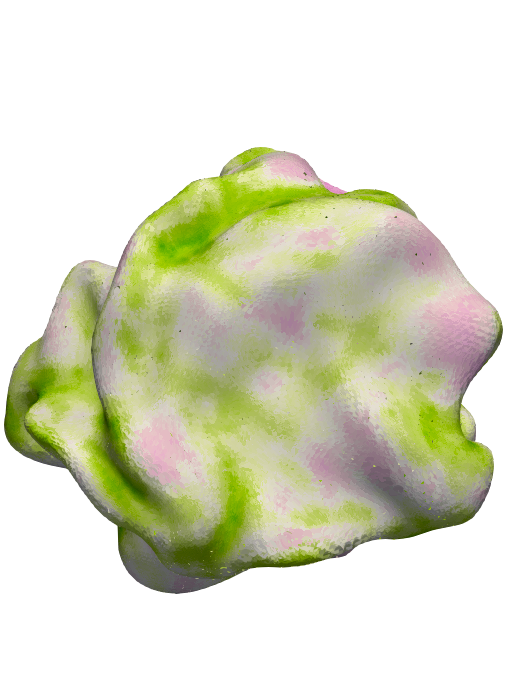
\includegraphics[height=0.45\figurewidth]{figures/spherical_time_1_7e-4_density_factor}};%
            \end{scope}
            \draw[thick, dashed, shorten <=1.7cm, shorten >=2.2cm] (-2.0, -3.5) -- (2.0, 3.5);
        \end{tikzpicture}
    };
    \node[label, yshift=1.3cm] at (image2.south) {$\begin{aligned}t &= \SI{1.7e-4}{\second} \\ N&=\num{140}\si{\kilo}\end{aligned}$};

    \node[image, below=of image1] (image3)
    {
        \begin{tikzpicture}
            \node[image] (base) {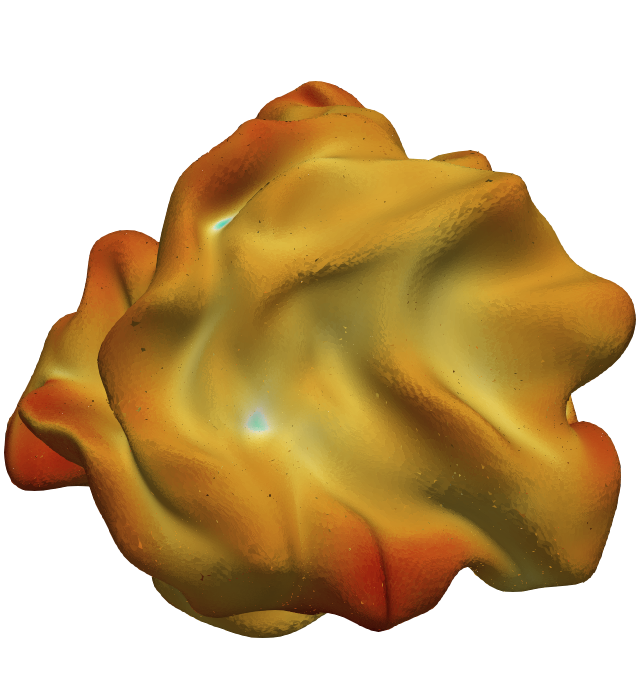
\includegraphics[height=0.45\figurewidth]{figures/spherical_time_2_4e-4}};%
            \begin{scope}
                \clip (base.south west) -- (base.north west) -- (base.north east) -- (base.south east) -- cycle;
                \clip (-2.0, -3.5) -- (2.0, 3.5) -- (4.0, 3.5) -- (4.0, -3.5)  -- cycle;
                \node[image] {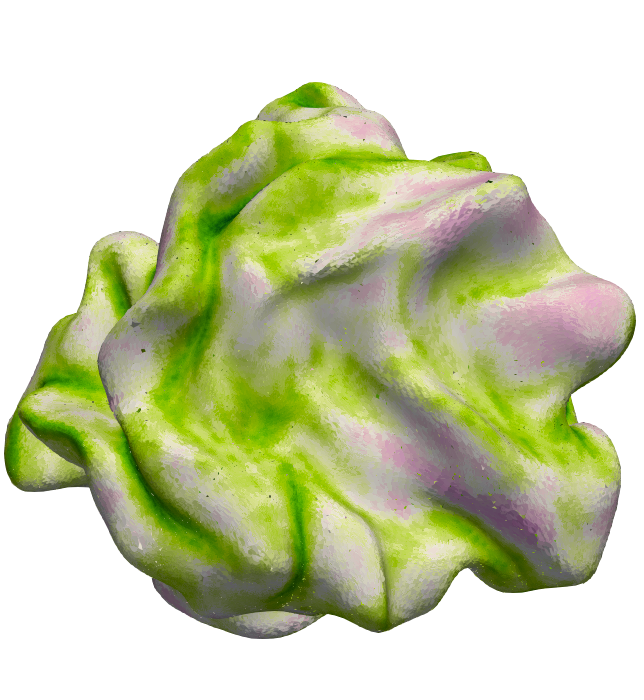
\includegraphics[height=0.45\figurewidth]{figures/spherical_time_2_4e-4_density_factor}};%
            \end{scope}
            \draw[thick, dashed, shorten <=1.4cm, shorten >=1.9cm] (-2.0, -3.5) -- (2.0, 3.5);
        \end{tikzpicture}
    };
    \node[label, yshift=0.5cm] at (image3.south) {$\begin{aligned}t &= \SI{2.4e-4}{\second} \\ N&=\num{400}\si{\kilo}\end{aligned}$};

    \node[image, right=of image3] (image4)
    {
        \begin{tikzpicture}
            \node[image] (base) {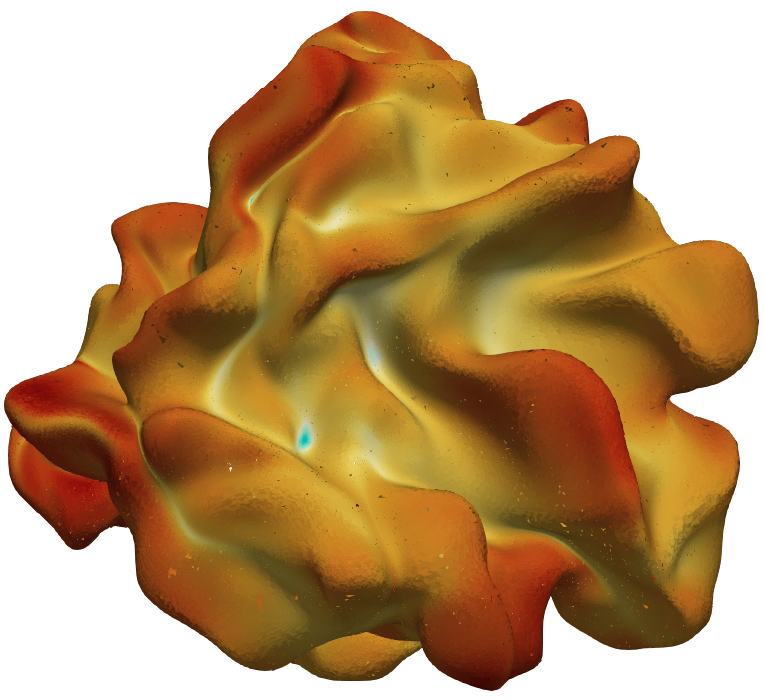
\includegraphics[height=0.45\figurewidth]{figures/spherical_time_3e-4}};%
            \begin{scope}
                \clip (base.south west) -- (base.north west) -- (base.north east) -- (base.south east) -- cycle;
                \clip (-2.0, -3.5) -- (2.0, 3.5) -- (4.0, 3.5) -- (4.0, -3.5)  -- cycle;
                \node[image] {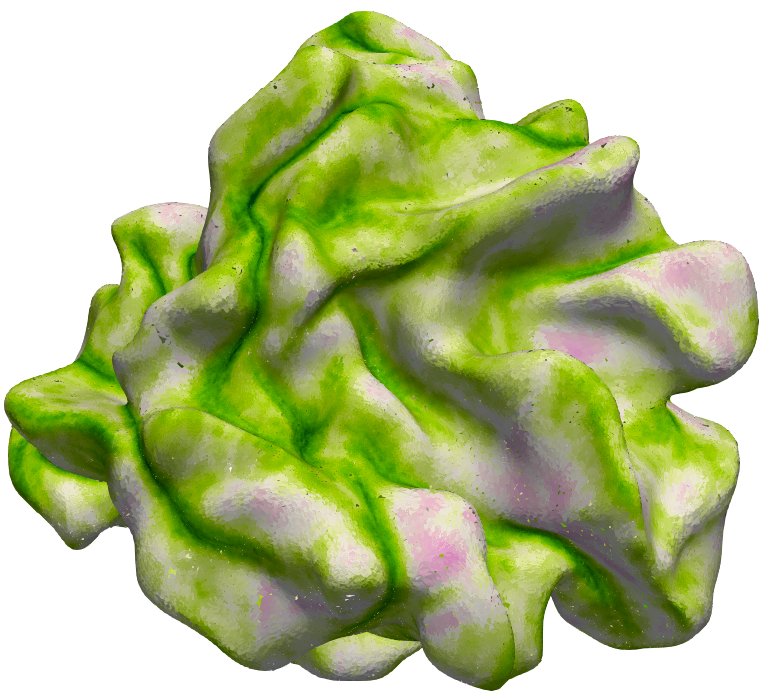
\includegraphics[height=0.45\figurewidth]{figures/spherical_time_3e-4_density_factor}};%
            \end{scope}
            \draw[thick, dashed, shorten <=1.05cm, shorten >=1.6cm] (-2.0, -3.5) -- (2.0, 3.5);
        \end{tikzpicture}
    };
    \node[label, yshift=0.5cm] at (image4.south) {$\begin{aligned}t &= \SI{3.1e-4}{\second} \\ N&=\num{870}\si{\kilo}\end{aligned}$};

    % \node (bbnw) at ($(image1.north west) + (-1.25, 0.4)$) {};
    % \node (bbse) at ($(image4.south east) + (1.35, -0.45)$) {};
    \coordinate (bottom) at ([yshift=-3cm]image4.south);

    \clip (image1.north west) rectangle (bottom -| image4.east);

    \node[anchor=north, yshift=-1.5cm, xshift=-3.5mm] at (image3.south){
        \begin{axis}[
        scale only axis,
        height=4cm,
        hide axis,
        domain=1.5:1.5,
        colorbar horizontal,
        colorbar/width=0.25cm,
        colormap name={cooltowarm_extended},
        point meta min=-1.5, point meta max=1.5,
        colorbar style={
            xlabel=\strut$c$,
            scaled ticks=false,
            xtick={-1, 0, 1},
            xticklabels={$10^{-1}$, $10^{\,0}$, $10^{\,1}$},
            % extra y ticks ={0.3, 0.4771212, 0.60206, 0.69897, 0.778151, 0.845098, 0.90309, 0.954242, 1.3, 1.4771212,
            %                 -0.3, -0.4771212, -0.60206, -0.69897, -0.778151, -0.845098, -0.90309, -0.954242, -1.3, -1.4771212},
            % extra y tick labels=\empty
        }]
      \end{axis}
    };
    \node[anchor=north, yshift=-1.5cm, xshift=-3.5mm] at (image4.south){
        \begin{axis}[
        scale only axis,
        height=4cm,
        hide axis,
        domain=-2.5:2.5,
        colorbar horizontal,
        colorbar/width=0.25cm,
        colormap name={green_purple},
        point meta min=-2.5, point meta max=2.5,
        colorbar style={
            xlabel=\strut$d$,
            scaled ticks=false,
            xtick={-2, -1, 0, 1, 2},
            xticklabels={$10^{-2}$, $10^{-1}$, $10^{\,0}$, $10^{\,1}$, $10^{\,2}$},
            % extra y ticks ={1, 1.3, 1.4771212, 1.60206, 1.69897, 1.778151, 1.845098, 1.90309, 1.954242,
            %                 -1, -1.3, -1.4771212, -1.60206, -1.69897, -1.778151, -1.845098, -1.90309, -1.954242},
            % extra y tick labels=\empty
        }]
      \end{axis}
    };
\end{tikzpicture}%

    %
\begin{tikzpicture}[
        font=\small,
        image/.style={anchor=center, inner sep=0, outer sep=0,
                      node distance = 1cm and 0,
                      minimum width=\figurewidth},
        label/.style={anchor=north, align=left}
    ]
    \pgfplotsset{colormap={cooltowarm_extended}{
    rgb=(0.12548999999999999, 0, 0.38039200000000001)
    rgb=(0.11372500000000001, 0.023529399999999999, 0.45097999999999999)
    rgb=(0.105882, 0.050980400000000002, 0.50980400000000003)
    rgb=(0.039215699999999999, 0.039215699999999999, 0.56078399999999995)
    rgb=(0.031372499999999998, 0.098039200000000007, 0.59999999999999998)
    rgb=(0.043137300000000003, 0.16470599999999999, 0.63921600000000001)
    rgb=(0.054901999999999999, 0.24313699999999999, 0.67843100000000001)
    rgb=(0.054901999999999999, 0.31764700000000001, 0.70980399999999999)
    rgb=(0.050980400000000002, 0.39607799999999999, 0.74117599999999995)
    rgb=(0.039215699999999999, 0.466667, 0.76862699999999995)
    rgb=(0.031372499999999998, 0.53725500000000004, 0.78823500000000002)
    rgb=(0.031372499999999998, 0.61568599999999996, 0.81176499999999996)
    rgb=(0.023529399999999999, 0.70980399999999999, 0.83137300000000003)
    rgb=(0.050980400000000002, 0.80000000000000004, 0.85097999999999996)
    rgb=(0.070588200000000004, 0.85490200000000005, 0.87058800000000003)
    rgb=(0.26274500000000001, 0.90196100000000001, 0.86274499999999998)
    rgb=(0.42352899999999999, 0.94117600000000001, 0.87451000000000001)
    rgb=(0.57254899999999997, 0.96470599999999995, 0.83529399999999998)
    rgb=(0.65882399999999997, 0.98039200000000004, 0.84313700000000003)
    rgb=(0.764706, 0.98039200000000004, 0.86666699999999997)
    rgb=(0.82745100000000005, 0.98039200000000004, 0.88627500000000003)
    rgb=(0.91372500000000001, 0.98823499999999997, 0.93725499999999995)
    rgb=(1, 1, 1)
    rgb=(0.98823499999999997, 0.98039200000000004, 0.87058800000000003)
    rgb=(0.99215699999999996, 0.96470599999999995, 0.71372500000000005)
    rgb=(0.98823499999999997, 0.95686300000000002, 0.64313699999999996)
    rgb=(0.98039200000000004, 0.91764699999999999, 0.50980400000000003)
    rgb=(0.96862700000000002, 0.87451000000000001, 0.40784300000000001)
    rgb=(0.94901999999999997, 0.82352899999999996, 0.32156899999999999)
    rgb=(0.92941200000000002, 0.77647100000000002, 0.27843099999999998)
    rgb=(0.90980399999999995, 0.71764700000000003, 0.235294)
    rgb=(0.89019599999999999, 0.65882399999999997, 0.196078)
    rgb=(0.87843099999999996, 0.61960800000000005, 0.168627)
    rgb=(0.87058800000000003, 0.54901999999999995, 0.156863)
    rgb=(0.85097999999999996, 0.47450999999999999, 0.145098)
    rgb=(0.83137300000000003, 0.41176499999999999, 0.13333300000000001)
    rgb=(0.81176499999999996, 0.34509800000000002, 0.11372500000000001)
    rgb=(0.78823500000000002, 0.26666699999999999, 0.094117599999999996)
    rgb=(0.74117599999999995, 0.18431400000000001, 0.074509800000000001)
    rgb=(0.69019600000000003, 0.12548999999999999, 0.062745099999999998)
    rgb=(0.61960800000000005, 0.062745099999999998, 0.043137300000000003)
    rgb=(0.54901999999999995, 0.027451, 0.070588200000000004)
    rgb=(0.47058800000000001, 0.0156863, 0.090196100000000001)
    rgb=(0.40000000000000002, 0.0039215700000000001, 0.101961)
    rgb=(0.34902, 0, 0.129412)
}}
    \pgfplotsset{colormap={green_purple}{
    rgb=(0.23137254901960799, 0, 0.34509803921568599)
    rgb=(0.337254901960784, 0, 0.44313725490196099)
    rgb=(0.44705882352941201, 0, 0.54117647058823504)
    rgb=(0.60392156862745106, 0.015686274509803901, 0.65098039215686299)
    rgb=(0.76470588235294101, 0.035294117647058802, 0.76470588235294101)
    rgb=(0.88235294117647101, 0.21568627450980399, 0.82352941176470595)
    rgb=(1, 0.50980392156862697, 0.90588235294117603)
    rgb=(1, 0.76470588235294101, 0.95294117647058796)
    rgb=(1, 1, 1)
    rgb=(0.85882352941176499, 0.94901960784313699, 0.49803921568627502)
    rgb=(0.71764705882352897, 0.90196078431372595, 0)
    rgb=(0.54117647058823504, 0.82745098039215703, 0)
    rgb=(0.36470588235294099, 0.752941176470588, 0)
    rgb=(0.25490196078431399, 0.64313725490196105, 0)
    rgb=(0.149019607843137, 0.53725490196078396, 0)
    rgb=(0.074509803921568599, 0.40000000000000002, 0.023529411764705899)
    rgb=(0, 0.26300000000000001, 0.050999999999999997)
}}
    \node[image] (image1)
    {
        \begin{tikzpicture}
            \node[image] (base) at (0,0) {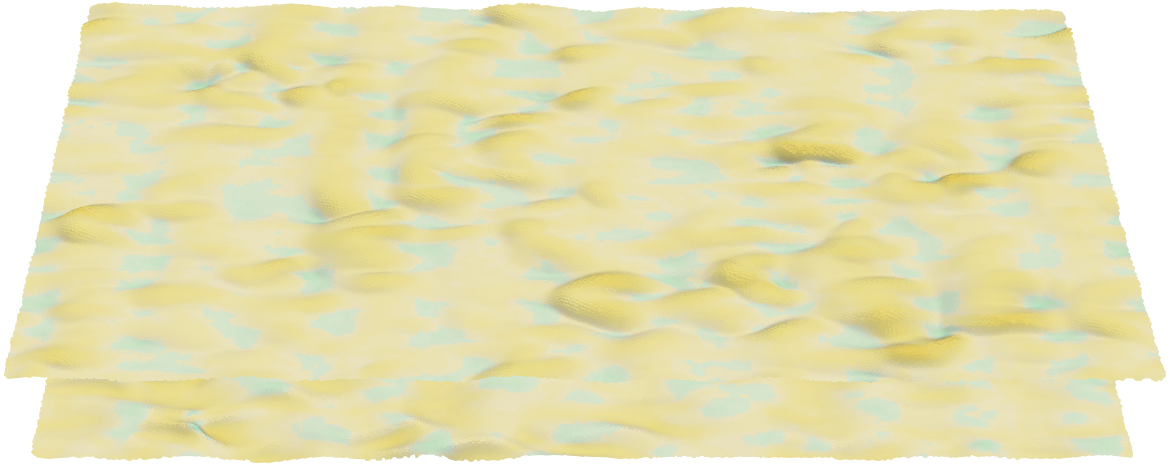
\includegraphics[width=0.8\figurewidth]{figures/hawkes_time_3e-5}};%
            \clip (base.south west) -- (base.north west) -- (base.north east) -- (base.south east) -- cycle;
            \clip (-2.0, -3.5) -- (2.0, 3.5) -- (4.0, 3.5) -- (4.0, -3.5) -- cycle;
            \node[image] at (0,0) {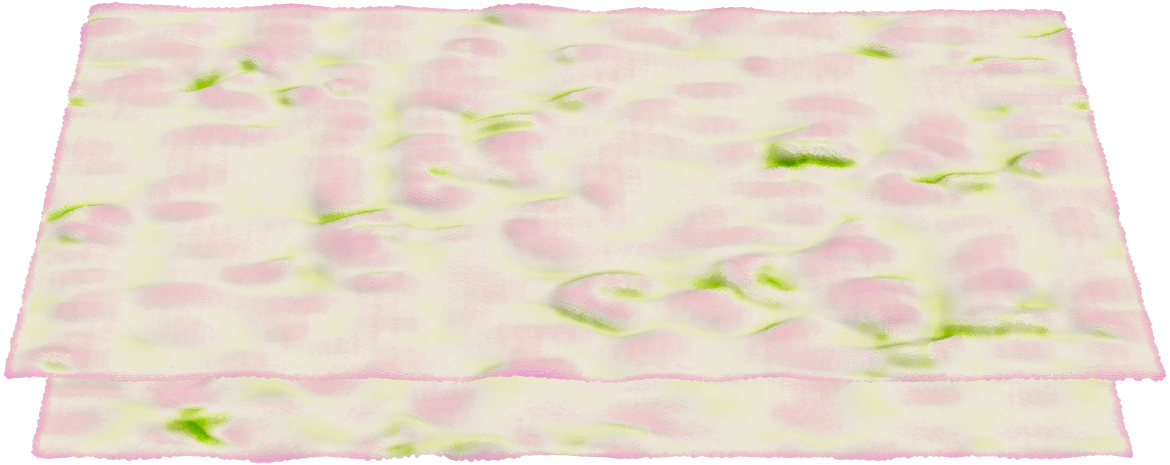
\includegraphics[width=0.8\figurewidth]{figures/hawkes_time_3e-5_density_factor}};%
        \end{tikzpicture}
    };
    \node[anchor=north, align=left] at (image1.south) {$t = \SI{3e-5}{\second} \quad N=\num{160}\si{\kilo}$};

    \node[image, below=of image1] (image2)
    {
        \begin{tikzpicture}
            \node[image] (base) at (0,0) {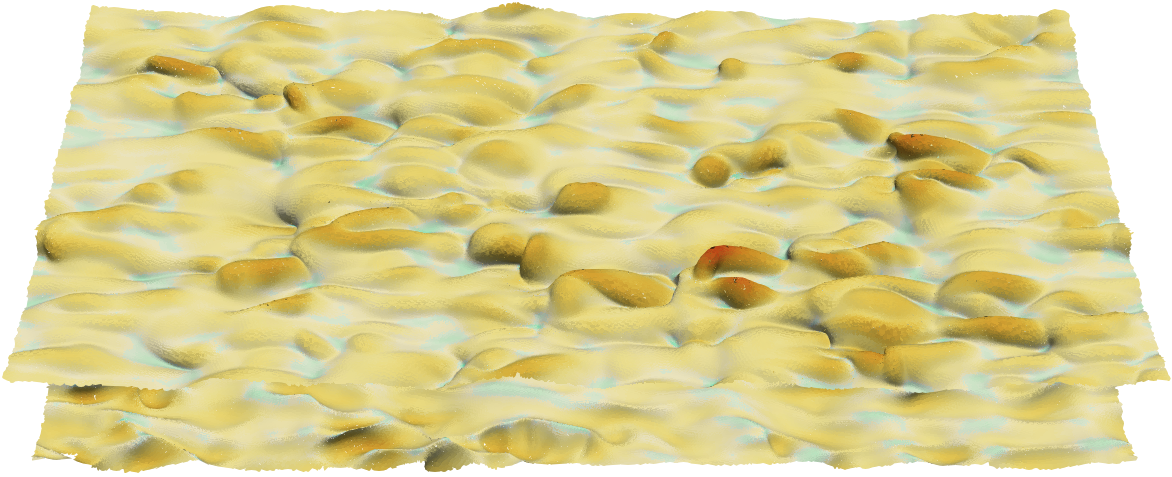
\includegraphics[width=0.8\figurewidth]{figures/hawkes_time_4e-5}};%
            \clip (base.south west) -- (base.north west) -- (base.north east) -- (base.south east) -- cycle;
            \clip (-2.0, -3.5) -- (2.0, 3.5) -- (4.0, 3.5) -- (4.0, -3.5) -- cycle;
            \node[image] at (0,0) {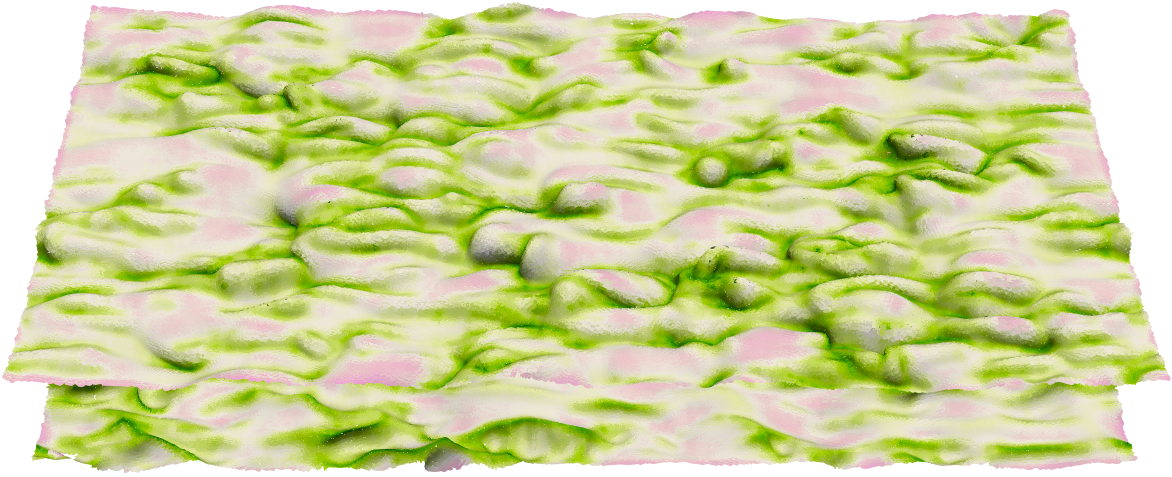
\includegraphics[width=0.8\figurewidth]{figures/hawkes_time_4e-5_density_factor}};%
        \end{tikzpicture}
    };
    \node[anchor=north, align=left] at (image2.south) {$t = \SI{4e-5}{\second} \quad N=\num{670}\si{\kilo}$};

    \node[image, below=of image2] (image3)
    {
        \begin{tikzpicture}
            \node[image] (base) at (0,0) {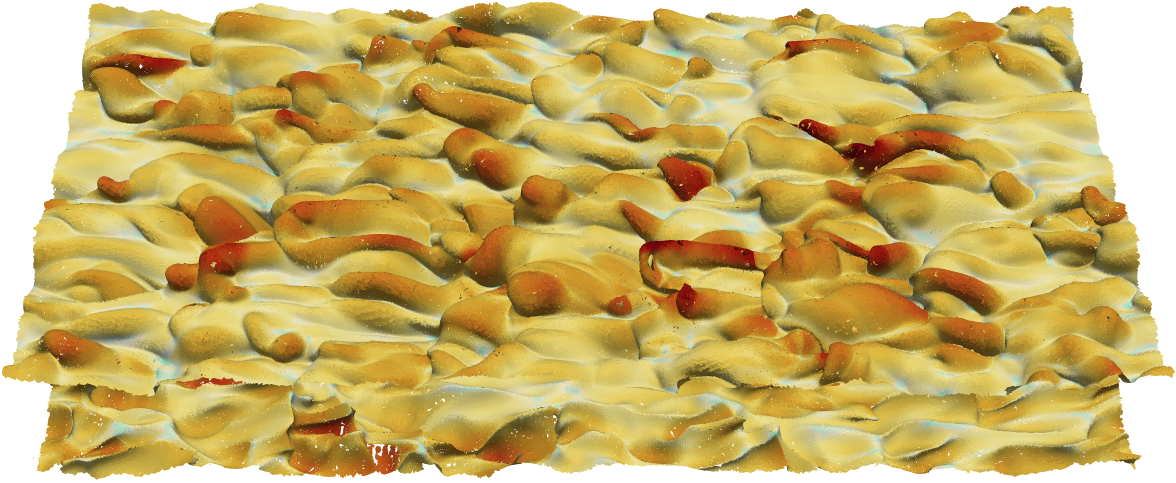
\includegraphics[width=0.8\figurewidth]{figures/hawkes_time_5e-5}};%
            \clip (base.south west) -- (base.north west) -- (base.north east) -- (base.south east) -- cycle;
            \clip (-2.0, -3.5) -- (2.0, 3.5) -- (6.0, 3.5) -- (6.0, -3.5) -- cycle;
            \node[image] at (0,0) {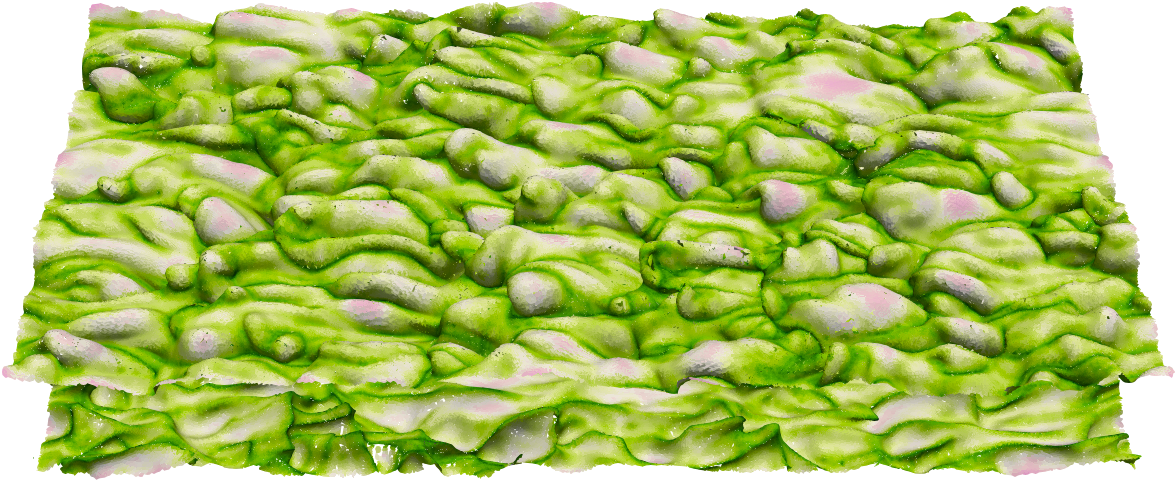
\includegraphics[width=0.8\figurewidth]{figures/hawkes_time_5e-5_density_factor}};%
        \end{tikzpicture}
    };
    \node[anchor=north, align=left] at (image3.south) {$t = \SI{5e-5}{\second} \quad N=\num{3000}\si{\kilo}$};

    \coordinate (bottom) at ([yshift=-2.5cm]image3.south);

    \clip (image1.north west) rectangle (image3.east |- bottom);

    \node[anchor=north east, yshift=-1cm, xshift=-6mm] at (image3.south){
        \begin{axis}[
        scale only axis,
        height=4cm,
        hide axis,
        domain=-2.5:2.5,
        colorbar horizontal,
        colorbar/width=0.25cm,
        colormap name={cooltowarm_extended},
        point meta min=-2.5, point meta max=2.5,
        colorbar style={
            xlabel=\strut$c$,
            scaled ticks=false,
            % yticklabel pos=left,
            xtick={-2, -1, 0, 1, 2},
            xticklabels={$10^{-2}$, $10^{-1}$, $10^{\,0}$, $10^{\,1}$, $10^{\,2}$},
            % extra y ticks ={0.3, 0.4771212, 0.60206, 0.69897, 0.778151, 0.845098, 0.90309, 0.954242, 1.3, 1.4771212,
            %                 -0.3, -0.4771212, -0.60206, -0.69897, -0.778151, -0.845098, -0.90309, -0.954242, -1.3, -1.4771212},
            % extra y tick labels=\empty
        }]
      \end{axis}
    };

    \node[anchor=north west, yshift=-1cm, xshift=-6mm] at (image3.south){
        \begin{axis}[
        scale only axis,
        height=4cm,
        hide axis,
        domain=-3:3,
        colorbar horizontal,
        colorbar/width=0.25cm,
        colormap name={green_purple},
        point meta min=-3, point meta max=3,
        colorbar style={
            xlabel=\strut$d$,
            scaled ticks=false,
            % yticklabel pos=right,
            xtick={-3, -2, -1, 0, 1, 2, 3},
            xticklabels={$10^{-3}$, $10^{-2}$, $10^{-1}$, $10^{\,0}$, $10^{\,1}$, $10^{\,2}$, $10^{\,3}$},
            % extra y ticks ={0.301, 0.4771212, 0.60206, 0.69897, 0.778151, 0.845098, 0.90309, 0.954242, 1, 1.3, 1.4771212, 1.60206, 1.69897, 1.778151, 1.845098, 1.90309, 1.954242, 2, 2.301, 2.4771212, 2.60206, 2.69897, 2.778151, 2.845098, 2.90309, 2.954242,
            %                 -0.301, -0.4771212, -0.60206, -0.69897, -0.778151, -0.845098, -0.90309, -0.954242, -1, -1.3, -1.4771212, -1.60206, -1.69897, -1.778151, -1.845098, -1.90309, -1.954242, -2, -2.301, -2.4771212, -2.60206, -2.69897, -2.778151, -2.845098, -2.90309, -2.954242},
            % extra y tick labels=\empty
        }]
      \end{axis}
    };
\end{tikzpicture}%

    \caption{
    Results of our algorithm for the real-world simulation cases. We show the
    stretch coefficient $c$ on a logarithmic scale. For the premixed
    flame case (top), $c$ was computed for an interval of $\Delta t =
    \SI{1.7e-4}{\second}$ and $\varepsilon_\shortparallel=0.02$. For
    the temporal diffusion jet case (bottom), we show the stretch coefficient
    since the start of the simulation, computed with
    $\varepsilon_\shortparallel=0.04$. We also show the number of micro-patches
    per surface area as a factor of the initial density at the start of the
    simulation. This density factor $d$ is also shown on a logarithmic scale.
    % \todo[inline]{fix size/layout}
    }
    \label{fig:simulation_results}
\end{figure}
%
As shown in Figures~\ref{fig:ground_truth_comparison} and
\ref{fig:ground_truth_errors}, the accuracy of our method is strongly
dependent on $r_\shortparallel$.
%
For large values of $r_\shortparallel$, the resulting deformation does not only
contain unreasonably large errors, but the surface also exhibits some holes.
%
Splitting too late means that there is potentially a lot of non-uniform
stretching across the patch that is not accounted for by the resulting child
patches.
%
This shows that observing only the normal error $e_\perp$ is not sufficient to
guarantee a good sampling of the surface, even if one is not interested in an
accurate result for the tangential deformation gradient.
%
As the error threshold decreases, the holes close and the stretching value
approaches the ground truth solution.
%
For the lowest error threshold value $r_\shortparallel = 0.01$, the number of
patches at the end is still one order of magnitude smaller than the number of
grid cells the function is resolved in.
%
% subsection analytic_test_function (end)
%
%
\subsection{Premixed Flame in a Box} % (fold)
\label{sub:premixed_flame_in_a_box}
%
We applied our algorithm to the combustion of a premixed hydrogen-air mixture in
a periodic box resolved in a $512 \times 512 \times 512$ regular grid.
%
A high-temperature hot spot is placed in the middle of the domain, which is
initialized with a flow field exhibiting isotropic turbulence.
%
After the gas mixture is ignited, a flame front travels through the domain,
consuming the fresh gas mixture and leaving burned products behind.
%
As the flame expands, it is deformed by the turbulent flow, which is in turn
influenced by the temperature and pressure changes induced by the chemical
reaction.
%
The flame surface of a premixed flame is often defined as an isosurface of the
temperature between the unburnt and burnt gases, which is what we track here.
%
Simulations of this type are relevant in safety research, where the influence of
the turbulence intensity on the ignition probability of the flame is studied.
%

%
The simulation ran for about \SI{90}{\hour} using \num{1024} parallel processors
and performing about \num{21000} iterations.
%
We chose $r_\perp = 0.1$ and $r_\shortparallel = 0.02$ as well as
$l_\perp = l_\shortparallel = \num{1e-4}$.
%
The thresholds $r_{\text{size}}$ and $t_{\text{size}}$ were chosen such that a
surface patch is always smaller than the smallest extent of a block of the
simulation domain, and larger than $\sfrac{1}{16}$ of the size of a grid cell.
%
\autoref{fig:simulation_results} (top) shows the results of our algorithm for
four snapshots of the simulation.
%
The simulation starts with a spherical configuration represented by about
\num{9000} micro-patches.
%
In the first shown time step, the surface has started to expand and wrinkle from
its initial configuration.
%
At this point, the surface is represented by about \num{50000} micro-patches.
%
Up until the last time step at $t=\SI{3.0e-4}{\second}$, the number of patches
increases to about \num{870000}.
%
Despite the change in surface area and complexity, we are able to accurately
track the surface without any neighbor information between micro-patches.
%
We obtain smooth results that show which regions of the surface have expanded or
contracted significantly.
%
%
\autoref{fig:simulation_results} shows the change in number of patches per
surface area compared to the initial seeding density.
%
A high concentration of patches occurs in areas with high surface curvature, as
well as in areas where the surface deformation has a large nonlinear component.
%

%
The ratio of the total surface area of all micro-patches to the true area of the
flame surface remains stably around \num{3.3} for the whole simulation.
%
This shows that our strategy for splitting and merging micro-patches is
successful in maintaining a consistent and stable coverage of the surface.
%
The number of splits performed per iteration fluctuates around
\SI{0.015}{\percent} of the total number of micro-patches at all times.
%
The number of merge events per iteration is almost zero up until the time
between the second and third snapshot shown in
\autoref{fig:simulation_results}, at iteration \num{15000}, where
it starts to increase, stabilizing at around half the number of splits.
%

%
% subsection premixed_flame_in_a_box (end)
%
\subsection{Temporal Diffusion Jet Flame} % (fold)
\label{sub:temporal_diffusion_jet_flame}
%
The second simulation is a temporal diffusion syngas jet flame resolved in a
$1024 \times 1025 \times 512$ regular grid.
%
In a diffusion flame, the fuel and oxidizer are not premixed before ignition,
such that combustion only takes place where the two gases mix.
%
The domain is initialized with a turbulent fuel layer in the center, surrounded
by a quiescent air co-flow.
%
The fuel layer and co-flow move in opposite directions, resulting in strong
shear forces that form vortices where the two gases meet.
%
The flame surface we track here is the isosurface of the stoichiometric mixture
fraction, which is the ratio between fuel and oxidizer that theoretically
results in perfect consumption of the fuel with no excess of the oxidizer.
%

%
The simulation ran for about \SI{23}{\hour} using \num{4096} parallel
processors.
%
In this time, the simulation performed about \num{3600} iterations.
%
For this case, we chose $r_\perp = 0.2$ and $r_\shortparallel = 0.04$ as well as
$l_\perp = l_\shortparallel = \num{1e-4}$.
%
The thresholds are chosen higher than in the premixed case, because here, we are
interested in the deformation of the surface over a smaller time interval of
$\SI{4e-5}{\second}$.
%
The thresholds $r_{\text{size}}$ and $t_{\text{size}}$ were chosen with the same
method employed for the premixed case.
%
We show our results for three different snapshots in
\autoref{fig:simulation_results} (bottom).
%
The case starts with a planar surface on both sides of the fuel jet, which is
moving from left to right in the images.
%
It is initially seeded with about \num{150000} micro-patches.
%
This number stays almost constant for the first \num{2000} iterations, as the
surface wrinkles only a very small amount.
%
After this, the surface starts deforming rapidly.
%
As a result, the number of micro-patches increases rapidly up to about 3 million
at the end of the simulation.
%
The surface deformation is characterized by lots of small fuel pockets intruding
into the opposing air flow.
%
These pockets are round and smooth towards the outside, while they form a lot of
sharp angles towards the inside.
%
Both the significant expansion of surface area at the tip of these pockets as
well as the sharp angles towards the fuel side are handled well by our
algorithm.
%
The ratio of the total area of all micro-patches to the true surface area
remains constant here as well, but on a slightly lower level of \num{3.15}.
%
The number of splits is almost zero until the surface starts to deform
significantly around iteration \num{2000}.
%
At this point, it starts to increase from \SI{0.002}{\percent} to about
\SI{0.003}{\percent} of the total number of micro-patches until the end of the
simulation.
%
This number is much smaller than for the premixed case, because here, the
surface area does not change so dramatically over time.
%
The number of merges is initially much smaller than the number of splits, but
increases steadily throughout the simulation until it is at about
\SI{75}{\percent} towards the end.
%
This is due to the contracting behavior near the sharp angles in between fuel
pockets, which causes lots of small patches to accumulate in a small area.
%
% subsection temporal_diffusion_jet_flame (end)
%
\subsection{Performance} % (fold)
\label{sub:fst_performance}
%
\autoref{fig:performance_spherical} shows the performance over the course of the
simulation, as well as the number of micro-patches existing at each time step.
%
We conducted multiple experiments with different choices for the subdivision
treshold $\varepsilon_\shortparallel$.
%
For the sake of brevity, we only discuss the results for the lowest choice of
$\varepsilon_\shortparallel$, which causes the highest overhead in computing
time and shows the most accurate results.
%

%
At the start of the premixed flame case, our implementation causes an overhead
in computing time of about \SI{300}{\milli\second} per iteration, or about
\SI{3}{\percent} of the base computing time.
%
As the flame surface expands, the overhead gradually increases, until it is at
about \SI{12.5}{\second} or \SI{130}{\percent} at the end of the simulation.
%
For the temporal diffusion jet, the overhead starts out at about
\SI{1200}{\milli\second} per iteration, or about \SI{10}{\percent} of the base
computing time.
%
It remains fairly constant for the first \num{1500} iterations, as the surface
does not change much during that time.
%
The surface then starts to wrinkle significantly, resulting in a sharp rise of
computing time, reaching up to \SI{42}{\second}, or about \SI{350}{\percent} of
the base time.
%
The overhead in computing time is proportional to the number of surface patches.
%
This means that it is also strongly dependent on the shape, area and deformation
of the flame surface, which will be different for each simulation case.
%
For the premixed flame case, our implementation generates an overhead of about
\SI{30}{\hour} or \SI{50}{\percent} for the whole simulation.
%
The memory consumption behaves very similarly, as it is also directly dependent
on the number of micro-patches.
%
At the start of the simulation, we consume about \SI{90}{\giga\byte} of
additional memory, which is an overhead of about \SI{30}{\percent} for this
simulation case.
%
This rises to about \SI{400}{\giga\byte} at the end of the simulation, which
represents an overhead of about \SI{130}{\percent}.
%
The total overhead in computing time caused by the temporal jet case is
\SI{8.4}{\hour} or about \SI{67}{\percent}.
%
The additional memory consumption here reaches from \SI{800}{\giga\byte} to
\SI{1800}{\giga\byte}, or \SI{44}{\percent} to \SI{150}{\percent}.
%

%
\begin{figure}
    \centering
    \setlength\figurewidth\linewidth
    \definecolor{tlowcolor}{HTML}{BD0026}
    \definecolor{tmidcolor}{HTML}{F03B20}
    \definecolor{thighcolor}{HTML}{FD8D3C}
    \definecolor{nlowcolor}{HTML}{253494}
    \definecolor{nmidcolor}{HTML}{2C7FB8}
    \definecolor{nhighcolor}{HTML}{41B6C4}
    %
%
\begin{tikzpicture}[
    t_low/.style={thick, tlowcolor},
    t_mid/.style={thick, tmidcolor},
    t_high/.style={thick, thighcolor},
    t_base/.style={thick, tlowcolor, dashed},
    n_low/.style={thick, nlowcolor},
    n_mid/.style={thick, nmidcolor},
    n_high/.style={thick, nhighcolor}
]
    \pgfplotsset{
        small,
        title style={
            font=\scshape,
            at={(0.5, 1)},
            anchor=north,
            inner sep=0pt,
            yshift=-3mm,
        },
        width=0.9\figurewidth,
        height=0.6\figurewidth,
        tick align=inside,
        every tick/.style={color=black, thin},
        tick pos=both,
        tick scale binop=\times,
        every y tick scale label/.style={
            at={(yticklabel* cs:1)},
            anchor=north west,
            inner sep=0pt,
            xshift=2.5pt
        },
        no markers,
        enlargelimits=true,
        ymin=0
    }

    \begin{axis}[
        name=spherical_np,
        title={\colorbox{white}{Premixed Flame}},
        % each nth point=100,
        ylabel={\color{nlowcolor}{$N$}},
        xlabel={Iterations},
        extra x ticks={7178, 12285, 17102, 21616},
        extra x tick style={
            grid=major,
            xticklabels={,,}
        },
        every x tick scale label/.style={
            at={(xticklabel* cs:1)},
            anchor=south east,
            inner sep=0pt,
            yshift=4pt
        },
        xtick={0, 5000, 10000, 15000, 20000},
        scaled y ticks=base 10:-5,
        scaled x ticks=base 10:-3,
        axis y line*=right,
        xticklabel pos=top,
        domain=0:21616,
        xmin=0,
        xmax=21616
    ]

        \addplot [n_high]
            coordinates{
                (200, 8621)
                (2106, 8621)
                (3000, 8629)
                (4581, 12747)
                (5000, 15213)
                (7000, 27691)
                (7178, 28638)
                (9000, 47493)
                (9762, 54925)
                (10000, 57434)
                (11000, 67515)
                (12285, 78572)
                (13000, 88204)
                (14732, 116516)
                (15000, 120911)
                (16000, 141969)
                (17102, 183076)
                (18000, 254563)
                (19397, 264183)
                (20000, 291308)
                (21000, 331552)
                (21616, 361552)
            };
        \label{plt:n_patches_0_1}

        \addplot [n_mid]
            coordinates{
                (200, 8621)
                (1000, 8621)
                (2000, 8621)
                (2106, 8621)
                (3000, 8657)
                (4000, 10292)
                (4581, 13229)
                (5000, 15914)
                (6000, 23281)
                (7000, 28752)
                (7178, 29694)
                (8000, 37741)
                (9000, 48633)
                (9762, 57080)
                (10000, 59875)
                (11000, 71951)
                (12000, 82838)
                (12285, 85716)
                (13000, 95742)
                (14000, 115402)
                (15000, 141836)
                (16000, 175734)
                (17000, 222679)
                (18000, 304182)
                (19000, 382856)
                (20000, 387671)
                (21000, 453553)
                (21616, 513311)
            };
        \label{plt:n_patches_0_05}

        \addplot [n_low]
            coordinates{
                (200, 8723)
                (1000, 9832)
                (2000, 12870)
                (2106, 13476)
                (3000, 18364)
                (4000, 24274)
                (4581, 28627)
                (5000, 32021)
                (6000, 40842)
                (7000, 49281)
                (7178, 50793)
                (8000, 57987)
                (9000, 68608)
                (9762, 79956)
                (10000, 84292)
                (11000, 104775)
                (12000, 130147)
                (13000, 164002)
                (14000, 205631)
                (14732, 242982)
                (15000, 258711)
                (16000, 321577)
                (17000, 388891)
                (18000, 464377)
                (19000, 553260)
                (20000, 657414)
                (21000, 780175)
                (21616, 867624)
            };
        \label{plt:n_patches_0_02}
    \end{axis}

    \begin{axis}[
        name=spherical_perf,
        at=(spherical_np.south west),
        anchor=south west,
        % each nth point=100,
        restrict y to domain=0.05:25,
        restrict x to domain=0:21616,
        unbounded coords=discard,
        xmin=0,
        xmax=21616,
        ylabel={\color{tlowcolor}{computing time/iteration [s]}},
        hide x axis,
        axis y line*=left,
    ]

        \addplot [t_base]
            table [
                skip first n=3,
                x index=0,
                y expr=\thisrowno{2}/1000,
            ] {figures/spherical_timings.txt};

        \addplot [t_high]
            table [
                skip first n=3,
                x index=0,
                y expr=(\thisrowno{2}+\thisrowno{3})/1000,
            ] {figures/spherical_timings_0_1.txt};

        \addplot [t_mid]
            table [
                skip first n=3,
                x index=0,
                y expr=(\thisrowno{2}+\thisrowno{3})/1000,
            ] {figures/spherical_timings_0_05.txt};

        \addplot [t_low]
            table [
                skip first n=3,
                x index=0,
                y expr=(\thisrowno{2}+\thisrowno{3})/1000,
            ] {figures/spherical_timings.txt};
    \end{axis}

    \matrix[
        anchor=north west,
        % draw,
        % fill=white,
        inner sep=0.2em,
        row sep=0.1em,
        column sep=0.1em,
        xshift=2mm,
        yshift=-2mm
      ]
      at (spherical_np.north west){
        \draw[t_low] (0,0.05cm) -- (0.4cm, 0.05cm); \draw[n_low] (0, -0.05cm) -- (0.4cm, -0.05cm); & \node[anchor=west, font=\small] {$\varepsilon_\shortparallel = 0.02$}; \\
        \draw[t_mid] (0,0.05cm) -- (0.4cm, 0.05cm); \draw[n_mid] (0, -0.05cm) -- (0.4cm, -0.05cm); & \node[anchor=west, font=\small] {$\varepsilon_\shortparallel = 0.05$}; \\
        \draw[t_high] (0,0.05cm) -- (0.4cm, 0.05cm); \draw[n_high] (0, -0.05cm) -- (0.4cm, -0.05cm); & \node[anchor=west, font=\small] {$\varepsilon_\shortparallel = 0.1$}; \\
        \draw[t_base] (0,0) -- (0.4cm, 0cm); & \node[anchor=west, font=\small] {Base}; \\
        };


    \begin{axis}[
        name=hawkes_np,
        title={\colorbox{white}{Temporal Diffusion Jet}},
        at=(spherical_np.south west),
        anchor=north west,
        yshift=-0.1cm,
        % each nth point=100,
        ylabel={\color{nlowcolor}{$N$}},
        xlabel={Iterations},
        xtick={0, 1000, 2000, 3000},
        ytick={0, 1000000, 2000000, 3000000},
        extra x ticks={1836, 2664, 3616},
        extra x tick style={
            grid=major,
            xticklabels={,,}
        },
        every x tick scale label/.style={
            at={(xticklabel* cs:1)},
            anchor=north east,
            inner sep=0pt,
            yshift=-1.5pt
        },
        scaled y ticks=base 10:-6,
        scaled x ticks=base 10:-3,
        axis y line*=right,
        xmax=3627,
        xmin=0,
        ymax=3200000
    ]
        \addplot [n_high]
            coordinates{
                (0, 151232)
                (1000, 151232)
                (2000, 154039)
                (2100, 157247)
                (2200, 162461)
                (2300, 171107)
                (2400, 184918)
                (2500, 207278)
                (2600, 235252)
                (2700, 269471)
                (2800, 315077)
                (2900, 369107)
                (3000, 424125)
                (3100, 478498)
                (3200, 537523)
                (3300, 605379)
                (3400, 678422)
                (3500, 757226)
                (3600, 841327)
                (3614, 852865)
            };

        \addplot [n_mid]
            coordinates{
                (0, 151232)
                (1000, 151232)
                (1500, 151250)
                (2000, 158181)
                (2100, 164851)
                (2200, 175599)
                (2300, 192543)
                (2400, 219452)
                (2500, 259674)
                (2600, 308258)
                (2700, 369591)
                (2800, 450016)
                (2900, 542517)
                (3000, 637255)
                (3100, 725948)
                (3200, 826107)
                (3300, 943111)
                (3400, 1063943)
                (3500, 1197164)
                (3600, 1345897)
                (3614, 1365405)
                % (3700, 1494575)
            };

        \addplot [n_low]
            coordinates{
                (0, 151232)
                (500, 151232)
                (637, 151232)
                (1000, 151232)
                (1192, 151232)
                (1500, 151536)
                (1834, 161858)
                (2000, 180865)
                (2200, 234132)
                (2500, 452623)
                (2663, 652381)
                (2700, 707504)
                (3000, 1285537)
                (3200, 1747570)
                (3616, 2976020)
            };
    \end{axis}

    \begin{axis}[
        name=hawkes_perf,
        at=(hawkes_np.south west),
        anchor=south west,
        % each nth point=25,
        restrict y to domain=0:60,
        restrict x to domain=0:3627,
        unbounded coords=discard,
        ylabel={\color{tlowcolor}{computing time/iteration [s]}},
        ytick={0, 25, 50},
        hide x axis,
        xmin=0,
        xmax=3627,
        ymax=57,
        axis y line*=left,
        legend pos=north west,
        legend cell align={left}
    ]
        \addplot [t_high]
            table [
                skip first n=0,
                x index=0,
                y expr=(\thisrowno{2}+\thisrowno{3})/1000,
            ] {figures/hawkes_timings_0_08.txt};

        \addplot [t_mid]
            table [
                skip first n=0,
                x index=0,
                y expr=(\thisrowno{2}+\thisrowno{3})/1000,
            ] {figures/hawkes_timings_0_06.txt};

        \addplot [t_low]
            table [
                skip first n=0,
                x index=0,
                y expr=(\thisrowno{2}+\thisrowno{3})/1000,
            ] {figures/hawkes_timings.txt};

        \addplot [t_base]
            table [
                skip first n=0,
                x index=0,
                y expr=\thisrowno{2}/1000,
            ] {figures/hawkes_timings.txt};
        % \addlegendentry{Base};
    \end{axis}

    \matrix[
        anchor=north west,
        % draw,
        % fill=white,
        inner sep=0.2em,
        row sep=0.1em,
        column sep=0.1em,
        xshift=2mm,
        yshift=-2mm
      ]
      at (hawkes_np.north west){
        \draw[t_low] (0,0.05cm) -- (0.4cm, 0.05cm); \draw[n_low] (0, -0.05cm) -- (0.4cm, -0.05cm); & \node[anchor=west, font=\small] {$\varepsilon_\shortparallel = 0.04$}; \\
        \draw[t_mid] (0,0.05cm) -- (0.4cm, 0.05cm); \draw[n_mid] (0, -0.05cm) -- (0.4cm, -0.05cm); & \node[anchor=west, font=\small] {$\varepsilon_\shortparallel = 0.08$}; \\
        \draw[t_high] (0,0.05cm) -- (0.4cm, 0.05cm); \draw[n_high] (0, -0.05cm) -- (0.4cm, -0.05cm); & \node[anchor=west, font=\small] {$\varepsilon_\shortparallel = 0.12$}; \\
        \draw[t_base] (0,0) -- (0.4cm, 0cm); & \node[anchor=west, font=\small] {Base}; \\
        };
\end{tikzpicture}
    \caption[Computing times per iteration for different subdivision thresholds
             $\varepsilon_\shortparallel$.]
            {\tikzset{external/export=false}
            Computing times per iteration for different subdivision thresholds
             $\varepsilon_\shortparallel$. We show the base computing time of
             the simulation without surface tracking (
             \tikz[baseline=-0.5ex]{\draw[thick, dashed, tlowcolor] (0, 0) -- (0.4cm, 0);})
             as well as the total times with our method enabled (
             \begin{tikzpicture}
                \draw[thick, tlowcolor] (0, 0.5ex) -- (0.4cm, 0.5ex);
                \draw[thick, tmidcolor] (0, 0) -- (0.4cm, 0);
                \draw[thick, thighcolor] (0, -0.5ex) -- (0.4cm, -0.5ex);
             \end{tikzpicture}
             ). The number $N$ of micro-patches over time is shown as context
             information (
             \begin{tikzpicture}
                \draw[thick, nlowcolor] (0, 0.5ex) -- (0.4cm, 0.5ex);
                \draw[thick, nmidcolor] (0, 0) -- (0.4cm, 0);
                \draw[thick, nhighcolor] (0, -0.5ex) -- (0.4cm, -0.5ex);
             \end{tikzpicture}
             ). The vertical lines mark the snapshots
             shown in \autoref{fig:simulation_results}.
             \tikzset{external/export=true}
    }
    \label{fig:performance_spherical}
    \Todo[inline]{fix positions of axis scaling labels}
\end{figure}
%

%
If we were to implement our approach as a post-processing step, we would need to
store the raw simulation data to disk, possibly transfer it over a network, and
read it again for each time step.
%
If we only store the simulation variables that are directly needed for tracking
the flame surface (flow velocity and one scalar variable), we would already need
\SI{100}{\tera\byte} of storage space for the whole premixed flame case, and
\SI{60}{\tera\byte} for the temporal jet case.
%
This is more than is typically available for a user or project on a current high
performance computing cluster.
%
Additionally, writing this data to disk for every simulation time step alone
would incur about \SI{21}{\hour} of run time on our computing cluster for the
premixed case and about \SI{13}{\hour} for the temporal jet case.
%
If we write all simulation variables, this increases to
\SI{420}{\tera\byte} (\SI{90}{\hour}) and \SI{320}{\tera\byte} (\SI{70}{\hour}),
respectively.
%
Considering that this is just part of the overhead inherent to a post-processing
approach makes it clear that an on-the-fly solution is the only way of obtaining
results with reasonable effort.
%

% subsection performance (end)
%
% section results (end)
